\documentclass[12pt]{article}

\usepackage{geometry}
\geometry{
	letterpaper,
	left = 0.75in,
	right = 0.75in,
	bottom = 1in,
	top = 1in }

\usepackage[english]{babel}
\usepackage{tabulary}
\usepackage{subfig}
\usepackage{float, graphicx}
\graphicspath{ {./gpx/} }

\title{Input Shaper Autocalibration using an OctoPrint Plugin}
\author{Ulendo}
\date{\vspace{-5ex}} % Hide the date that will be part of maketitle.

\begin{document}

\maketitle

\section{Requirements}
This version requires the following:
\begin{itemize}
	\item A Raspberry Pi single-board computer (SBC) running Octoprint and this plugin.
	\item An ADXL345 accelerometer wired to the SBC.
	\item Compatible firmware on the printers connected to the SBC.
\end{itemize}

\section{Accelerometer Setup}
The accelerometer should be wired to the SBC as in Figure \ref{fig:accelerometer_wiring_old.png}.
\begin{figure}[H]
	\centering
	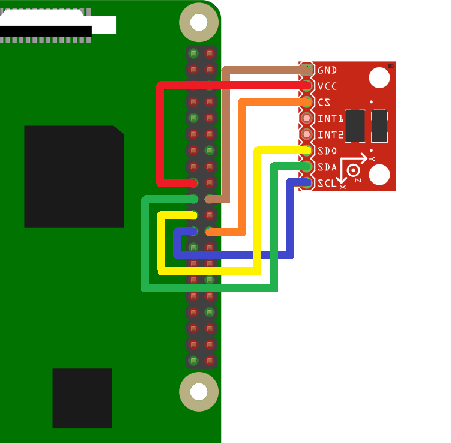
\includegraphics[width=0.3\linewidth]{accelerometer_wiring_old.png}
	\caption{Accelerometer wiring.}
	\label{fig:accelerometer_wiring_old.png}
\end{figure}
The accelerometer needs to be mounted on the axis being calibrated aligned according to the axes labeling on the acclerometer (Figure \ref{fig:accelerometer_axes.png}). The orientation of the accelerometer does not matter provided the axis in motion is aligned with the arrow of the axis label on the acclerometer.
\begin{figure}[H]
	\centering
	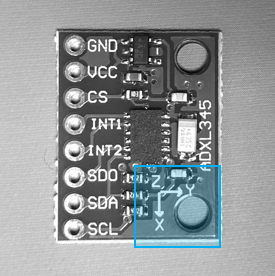
\includegraphics[width=0.3\linewidth]{accelerometer_axes.png}
	\caption{Accelerometer axes label.}
	\label{fig:accelerometer_axes.png}
\end{figure}
An example of good mounting locations on the LulzBot TAZ Pro are shown in Figure \ref{fig:tazpro_mounting}. If the axis being calibrated is moving the hotend, mounting the accelerometer closer to the nozzle will yield better results. If the axis being calibrated is moving a bed, the accelerometer should be placed on the bed and not near any edge of the bed.
% NOTE: The '%' suppresses whitespace at the line.
\begin{figure}[H]%
    \centering
    \subfloat[\centering X Mounting]{{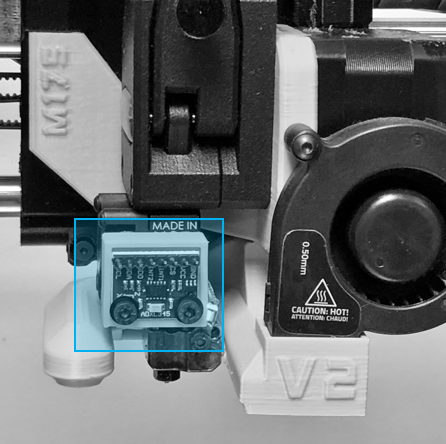
\includegraphics[height=7cm]{accelerometer_on_tazpro_x.png} }}%
    \qquad
    \subfloat[\centering Y Mounting]{{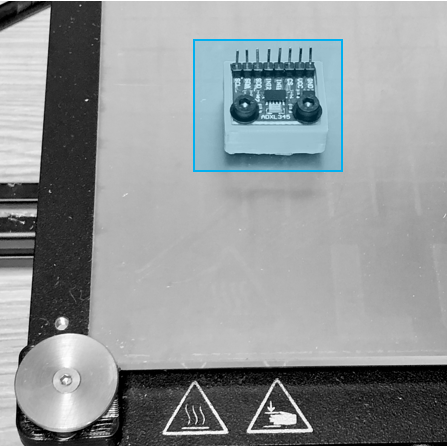
\includegraphics[height=7cm]{accelerometer_on_tazpro_y.png} }}%
    \caption{Mounting on LulzBot TAZ Pro.}%
    \label{fig:tazpro_mounting}%
\end{figure}


\section{Using the Plugin}
\begin{itemize}
	\item The plugin interface is available as a tab under the main OctoPrint user interface. (Figure \ref{fig:plugin_005.png}).
		\begin{figure}[H]
			\centering
			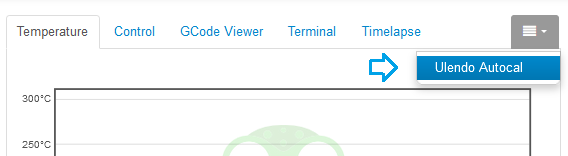
\includegraphics{plugin_005.png}
			\caption{Plugin tab.}
			\label{fig:plugin_005.png}
		\end{figure}
	\item To begin, click the Connect Accelerometer button. The accelerometer will be connected and tested. If successful, the button will turn green and the calibration buttons will be enabled (Figure \ref{fig:plugin_006.png}). A graph at the top of the tab will display in real time any accelerometer data that is being collected (Figure \ref{fig:plugin_006.png}, blue).
		\begin{figure}[H]
			\centering
			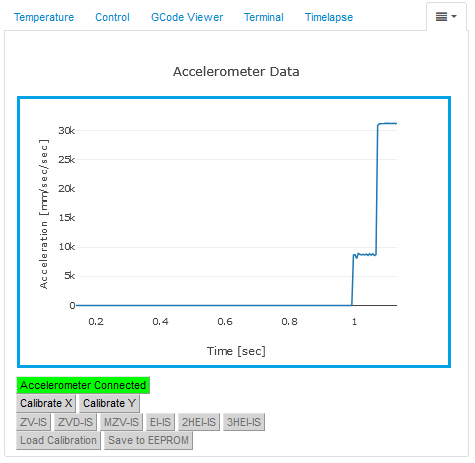
\includegraphics{plugin_006.png}
			\caption{Accelerometer connection data.}
			\label{fig:plugin_006.png}
		\end{figure}
	\item Verify the accelerometer is mounted on the correct axis, and that motion (in particular, homing of the axis) will clear the sensor and its wiring. Then, click Calibrate X or Calibrate Y to begin calibrating the desired axis. A prompt (Figure \ref{fig:plugin_007.png}) will display asking to verify the motion is clear. Click Proceed when ready.
		\begin{figure}[H]
			\centering
			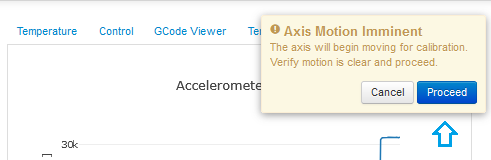
\includegraphics{plugin_007.png}
			\caption{Verification popup.}
			\label{fig:plugin_007.png}
		\end{figure}
	\item Once the routine is complete, if successful, the shaper algorithm buttons will enable. Clicking one will display a graph with the response of the printer at various frequencies both before and after the input shaping will be applied (Figure \ref{fig:plugin_008.png}).
		\begin{figure}[H]
			\centering
			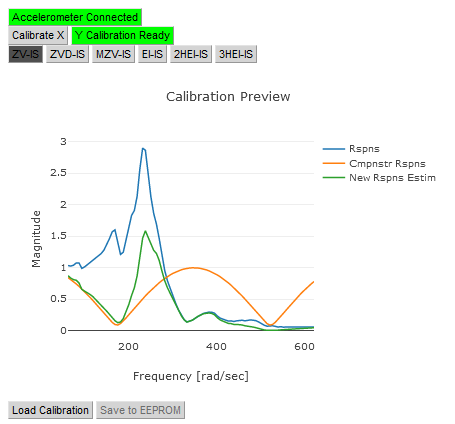
\includegraphics{plugin_008.png}
			\caption{Calibration results.}
			\label{fig:plugin_008.png}
		\end{figure}
	\item The extra-insensitive (EI) shapers will have a vibration tolerance parameter that can be specified by the user. It may be modified using the slider at the bottom of the graph as in Figure \ref{fig:plugin_009.png}; the default value is 5\%. Once an input shaper has been selected, click the Load Calibration to send the parameters to the printer. A verification routine is run.
		\begin{figure}[H]
			\centering
			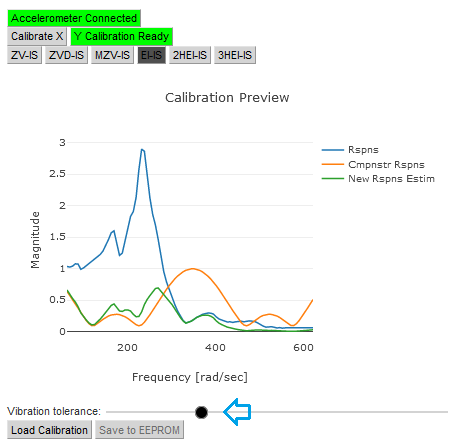
\includegraphics{plugin_009.png}
			\caption{EI input shaper selection.}
			\label{fig:plugin_009.png}
		\end{figure}
	\item Once the verification routine is a complete, a final graph will show the results of the input shaping algorithm tested on the machine (Figure \ref{fig:plugin_010.png}). At this point the printer is configured \textbf{for this session} with the selected input shaper and the parameters determined by the autocalibration service. Printing or other normal operations can resume, however a power cycle will reset the shaper settings.
		\begin{figure}[H]
			\centering
			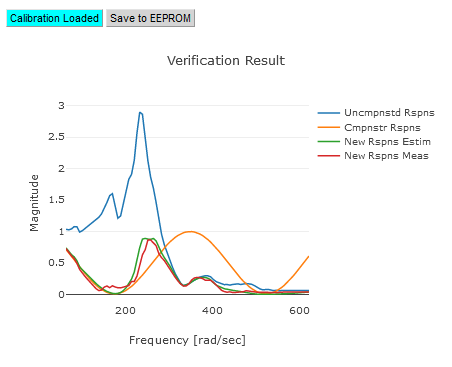
\includegraphics{plugin_010.png}
			\caption{Verification results.}
			\label{fig:plugin_010.png}
		\end{figure}
	\item If ready to save the settings to the printer, click the Save to EEPROM button (Figure \ref{fig:plugin_011.png}).  Now, these settings will persist across power cycles.
		\begin{figure}[H]
			\centering
			
\includegraphics{plugin_011.png}
			\caption{Save to EEPROM button.}
			\label{fig:plugin_011.png}
		\end{figure}
\end{itemize}

\section{Troubleshooting}
Common faults will be diagnosed and if detected a popup may give information such as in Figure \ref{fig:plugin_012.png}. A user should try any corrective actions suggested by the popup. If unable to resolve, please contact Ulendo.
	\begin{figure}[H]
		\centering
		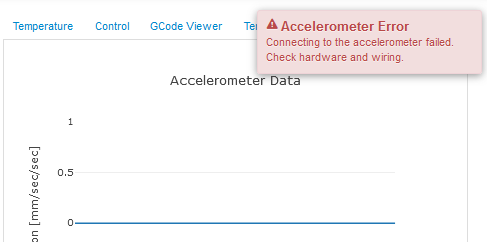
\includegraphics{plugin_012.png}
		\caption{Fault popup.}
		\label{fig:plugin_012.png}
	\end{figure}

\section{Suggestions}
\begin{itemize}
	\item At present the service does not recommend an input shaper algorithm. Ulendo suggests starting with the "ZVD" input shaper. If rounding is excessive, try "ZV"; if too much ringing remains, try the others in the order they appear on the screen.
	\item The vibration tolerance parameter can be left at its default (5\%). It may be increased to sacrifice performance to provide more consistent results in the case of changing environment (e.g.: due to printer component wear), or decreased to improve performance but be more sensitive to such changes.
\end{itemize}


\section{Known Issues}
\begin{itemize}
	\item The plugin does not currently check if the printer is busy before issuing commands. Therefore, verify the printer is idling before using the plugin.
\end{itemize}

\end{document}